\newpage
\section{Data Link Layer}
\subsection{Overview of Data link layer}
\subsubsection{The Design Principles of the Data Link Layer}

To achieve reliable and efficient communication between two adjacent machines

Three main functions of the data link layer:
\begin{itemize}
    \item Framing: Break stream of bits up into discrete frames
    \item Error control: Error Detection and Error Correction
    \item Flow control: to prevent a sender to overload the receiver with packets
\end{itemize}

\subsubsection{Position of the Data Link Layer}
\begin{figure}[!htb]
    \centering
    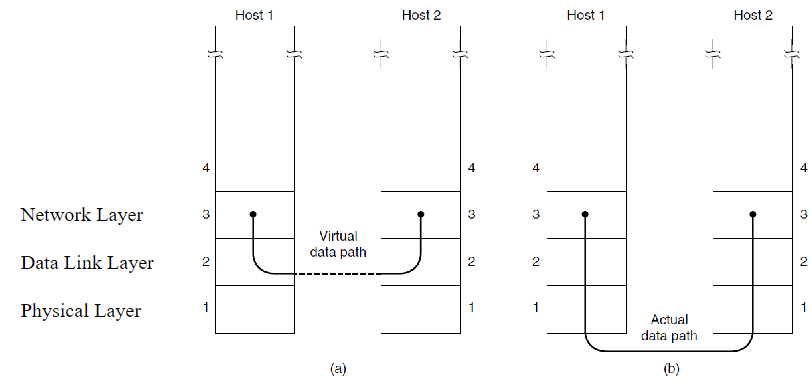
\includegraphics[width=0.42\textwidth]{pic/CN3/The function of the data link layer is to provide services to the network layer.}
    \caption{The function of the data link layer is to provide services to the network layer.}
\end{figure}

\subsubsection{The Services of Data Link Layer}
\begin{enumerate}
    \item Unacknowledged connectionless service
    \subitem for very low error-rate and real-time applications
    \subitem e.g. Ethernet
    \item Acknowledged connectionless service
    \subitem for unreliable channels
    \subitem e.g. 802.11 WiFi
    \item Acknowledged connection-oriented service
    \subitem for over long, unreliable links
    \subitem e.g. a satellite channel or a long-distance telephone circuit
\end{enumerate}

\subsection{Data link layer: Framing}
General Frame Format: a header, a payload field, and a trailer
\begin{figure}[!htb]
    \centering
    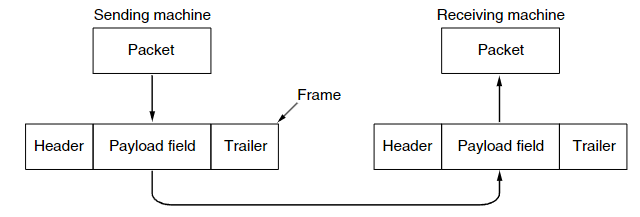
\includegraphics[width=0.42\textwidth]{pic/CN3/Relationship between packets and frames.}
    \caption{Relationship between packets and frames.}
\end{figure}

会加一些冗余的 bits 来降低 bit error rate. There are about four methods:
\begin{enumerate}
    \item Byte count: 若刚好 count 出错了就会很寄. 
    \item Flag bytes with byte stuffing: 因为 flag 可能会在传输数据中出现, 所以在其前加上 a special escape byte (ESC) 以区别, 若 ESC 也在数据中, 则同样其前加 ESC. 
    \begin{figure}[!htb]
        \centering
        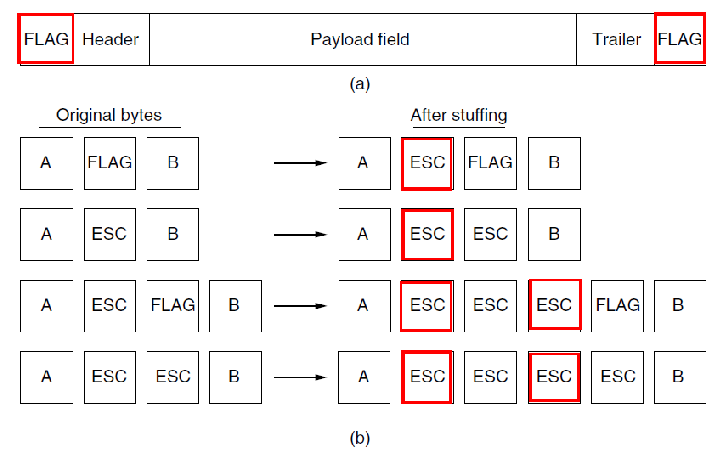
\includegraphics[width=0.42\textwidth]{pic/CN3/Flag Byte with Byte Stuffing.png}
        \caption{(a) A frame delimited by flag bytes. (b) Four examples of byte sequences before and after byte stuffing.}
    \end{figure}
    
    \item Flag bits with bit stuffing: Whenever the sender's data link layer encounters five consecutive 1s in the data, it automatically stuffs a 0 bit into the outgoing bit stream.
    \begin{figure}[!htb]
        \centering
        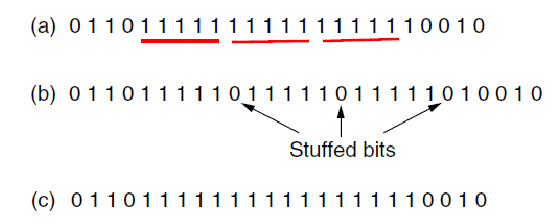
\includegraphics[width=0.309\textwidth]{pic/CN3/Flag Byte with Bit Stuffing.png}
        \caption{Bit stuffing. (a) The original data. (b) The data as they appear on the line. (c) The data as they are stored in the receiver's memory after destuffing.}
    \end{figure}
    
    \item Physical layer coding violations: We can use some reserved signals to indicate the start and the end frames.
\end{enumerate}

\subsection{Data link layer: Error Control}
\begin{itemize}
    \item Error-Correcting Codes: For unreliable channels
    \item Error-Detecting Codes: For highly reliable channels
\end{itemize}
the redundant bits that offer protection are as likely to be received in error as the data bits.

\subsubsection{Error Models of Communication Channels}

\subsubsection{Error Correction}
two different error-correcting codes:
\begin{itemize}
    \item Hamming codes
    \item Binary convolutional codes
\end{itemize}

对码本(一对码字), from this list to find the two codewords with the smallest Hamming distance. This distance is the Hamming distance of the complete code. (码本中码字间两两最小的 Hamming distance 是码本的 Hamming distance)

The code rate is $m/n$. (n=m+r, nis the total length of a block, r is redundance)

\begin{itemize}
    \item To reliably detect d errors, you need a distance d + 1 code
    \item To correct d errors, you need a distance 2d + 1 code.
\end{itemize}
we expect only single- or double-bit errors

For all single errors to be corrected, this requirement becomes
\begin{align*}
    (m+r+1)\le 2^r
\end{align*}
Given $m$, this puts a lower limit on the number of check bits needed to correct single errors. 

\paragraph{Hamming Code} $k$ data bits $+ (n - k)$ check bits. value 1 are XORed together to calculate the check bits.  %TODO 定义总结 P34-36

Convolutional Code: the original m bits do not appear % 不考, 摸了! P38-


\subsubsection{Error Detection}
three different error-detecting codes:
\begin{itemize}
    \item Parity: the number of 1 bits in the codeword is even or odd.
    \subitem Advantage: bit error rates 非常低时, 花费比 error correction 少
    \subitem Difficulty: for a long burst error (一大段错误), 仅能检测一般的错误. To against burst errors:
    \begin{itemize}
        \item Interleaving
        \begin{figure}[!htb]
            \centering
            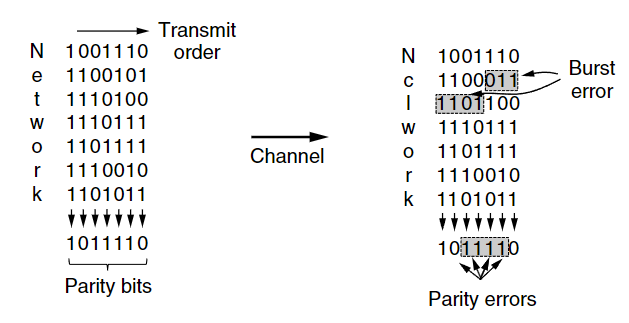
\includegraphics[width=0.309\textwidth]{pic/CN3/Interleaving}
            \caption{Interleaving of parity bits to detect a burst error}
        \end{figure}
        \item Two-dimensional parity
        \begin{figure}[!htb]
            \centering
            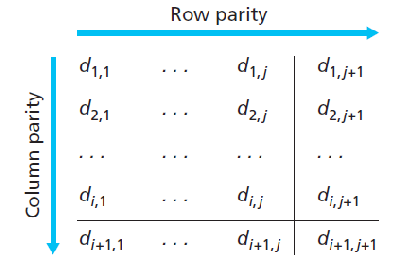
\includegraphics[width=0.309\textwidth]{pic/CN3/Two-dimensional parity}
            \caption{Two-dimensional parity}
        \end{figure}
        
    \end{itemize}
    \item Checksums: {\small
    \begin{itemize}
        \item One's complement has two representations of zero, all 0s and all 1s
        \item two's complement arithmetic
    \end{itemize}
    \subitem Sending:
    \begin{enumerate}
        \item Arrange data in 16-bit words
        \item Put zero in checksum position, add
        \item Add any carryover back to get 16 bits
        \item Negative (complement) to get sum
    \end{enumerate}
    \subitem Receiving
    \begin{enumerate}
        \item Arrange data in 16-bit words
        \item Checksum will be non-zero, add
        \item Add any carryover back to get 16 bits
        \item Negate the result and check it is 0.
    \end{enumerate} }
    \item Cyclic Redundancy Checks (CRCs): predetermined bit pattern - key (or the generator polynomial) (Both the high- and low-order bits of the generator must be 1)
    \begin{figure}[!htb]
        \centering
        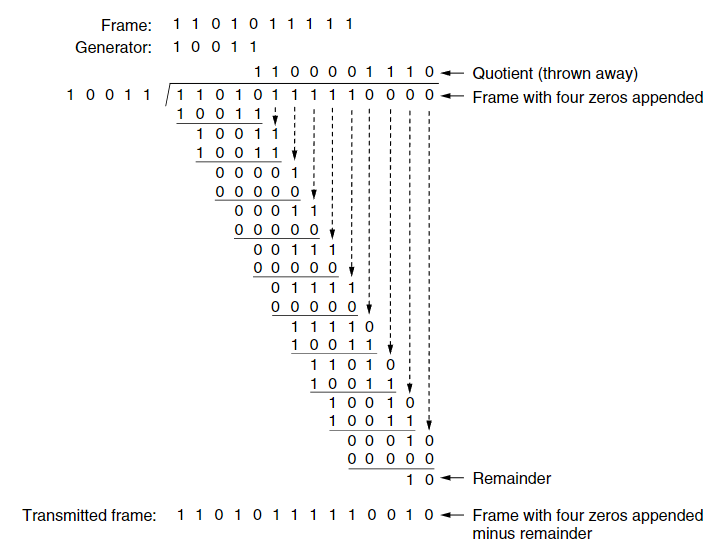
\includegraphics[width=0.309\textwidth]{pic/CN3/CRC.png}
        \caption{Example calculation of the CRC}
    \end{figure}
    
\end{itemize}


\subsection{Elementary data link protocols}
\subsubsection{A Utopian Simplex Protocol}
Unrealistic assumptions:
\begin{enumerate}
    \item Data are transmitted in one direction only.
    \item Both the transmitting and receiving network layers are always ready.
    \item Processing time can be ignored.
    \item Infinite buffer space is available.
    \item The communication channel between the data link layer never damages or loses frames.
\end{enumerate}

\subsubsection{A Simplex Stop-and-Wait Protocol for an Error-Free Channel}
This protocol is to tackle the problem of preventing the sender from flooding the receiver with frames faster than the latter is able to process them.

receiver provide a little dummy frame (an acknowledge frame) as feedback to sender (目的是告诉 sender, receiver 已完成接受).

\subsubsection{A Simplex Stop-and-Wait Protocol for a Noisy Channel}
To add a timer, the receiver would only send an acknowledgement frame if the data were correctly received. timer 触发但没收到 ack, sender 会重传. 

A fatal flaw: duplicate. 若 ack 完全丢失, 会接受一个 frame 两次, 不可接受. 

put a sequence number to avoid duplicate. the only ambiguity is between a frame and its immediate predecessor or successor

\begin{itemize}
    \item After transmitting a frame and starting the timer, the sender waits for something exciting to happen.
    \item Only three possibilities exist: an acknowledgement frame arrives undamaged, a damaged acknowledgement frame staggers in, or the timer expires.
\end{itemize}

\subsection{Sliding window protocols}
\subsubsection{Piggybacking(驮运)}
ack 可以搭顺风车, 与下一个数据包一起发送. The technique of temporarily delaying outgoing acknowledgements so that they can be hooked onto the next outgoing data frame. In effect, the acknowledgement gets a free ride on the next outgoing data frame.

使用一个计时器决定 ack 是否搭顺风车, 在时间内有其他包就顺风车, 没有就单独发. 

Sliding window bidirectional protocol(注意其不同点): 
\begin{itemize}
    \item A One-Bit Sliding Window Protocol (stop-and-wait)
    \item A Protocol Using Go Back N
    \item A Protocol Using Selective Repeat
\end{itemize}

\subsubsection{The Essence of All Sliding Window Protocols}
\paragraph{the sender}: maintains \textbf{a set of sequence numbers} corresponding to frames it is permitted to send. These frames are said to fall within the \textbf{sending window}.

The sequence numbers within the sender's window represents frames that 
\begin{enumerate}
    \item have been sent but are yet not acknowledged 
    \item can be sent
\end{enumerate}
(If some frames are lost or damaged in transit, the sender should prepare for possible retransmission)

If the window ever grows to its maximum size, the sending data link layer must forcibly shut off the network layer until another buffer becomes free.  --- \textbf{Flow Control}

\paragraph{the receiver}: also maintains \textbf{a receiving window} corresponding to the set of frames it is permitted to accept.

Any frame falling within the window is put in the receiver's buffer. Any frame falling outside the window is discarded.

When a frame whose sequence number is equal to the lower edge of the window is received, it is passed to the network layer and the window is rotated by one.

Note that a window size of 1 means that the data link layer only accepts frames in order. (For large window, it should answer how to keep the correct order)

The sender’s window and the receiver’s window need not have the same size. 

\begin{figure}[!htb]
    \centering
    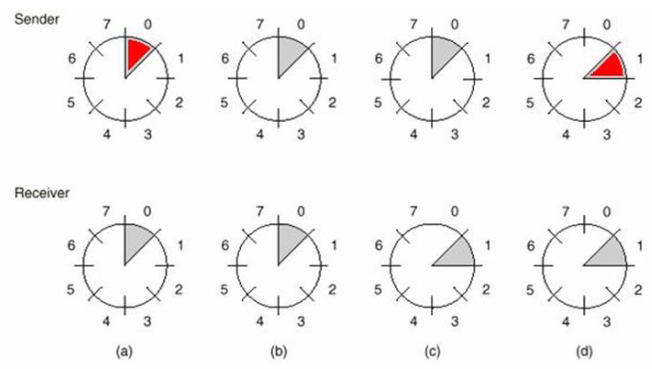
\includegraphics[width=0.42\textwidth]{pic/CN3/Sliding Window Protocols}
    \caption{A sliding window of size 1, with a 3-bit sequence number: (a) Initially. (b) After the first frame has been sent. (c) After the first frame has been received. (d) After the first acknowledgement has been received.}
\end{figure}

\subsubsection{One-Bit Sliding Window Protocol}%TODO 回去看代码, P88-
\begin{figure}[!htb]
    \centering
    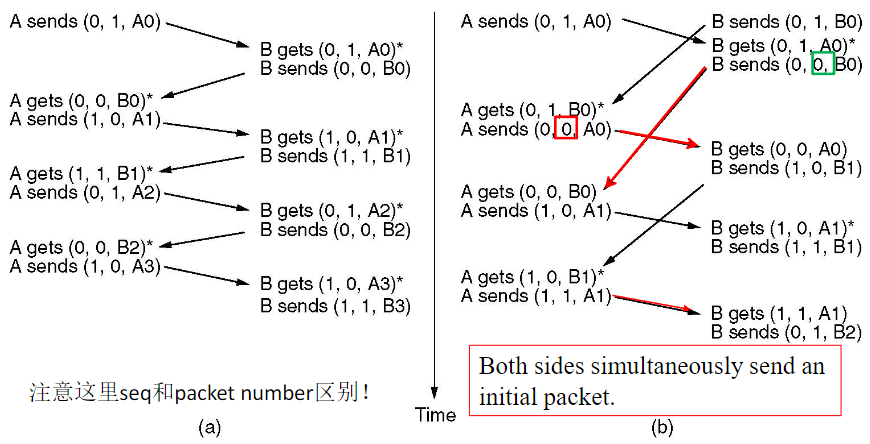
\includegraphics[width=0.42\textwidth]{pic/CN3/One-Bit Sliding Window Protocol}
    \caption{Two scenarios for protocol 4 (One-bit Sliding Window). (a) Normal case. (b) Abnormal case. The notation is (seq, ack, packet number). An asterisk indicates where a network layer accepts a packet. (Here the red arrows denotes the retransmissions because of timeout)}
\end{figure}

e.g. The rule requiring a sender to wait for an acknowledgement before sending another frame, 导致 bandwidth 利用率极低. The protocol 4 is disastrous in terms of efficiency under the situation of a long transit time, high bandwidth, and short frame length.

To find an appropriate value for $w$
\begin{enumerate}%TODO P92
    \item the bandwidth-delay product
    \item We can divide this quantity by the number of bits in a frame to express it as a number of frames. --- $BD$
    \item $w$ should be set to $2BD+1$
\end{enumerate}

\subsubsection{A Protocol Using Go Back N}
Pipelining frames over an unreliable channel raises some serious problem.
\begin{itemize}
    \item What happens if a frame in the middle of a long stream is damaged or lost?
    \item What should the receiver do with all the correct frames following a damaged frame?
\end{itemize}
Remember that the receiving data link layer is obligated to hand packets to the network layer in sequence.

\begin{figure}[!htb]
    \centering
    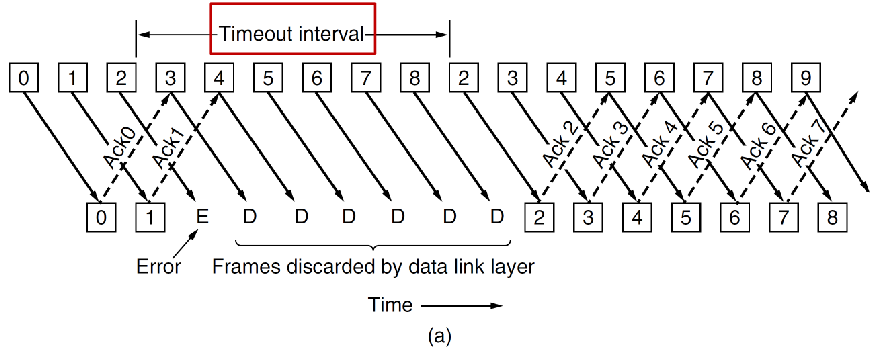
\includegraphics[width=0.42\textwidth]{pic/CN3/Receiver's window size is 1.}
    \caption{(a) Receiver's window size is 1. --- Go Back N}
    \label{fig:Go Back N}
\end{figure}
In \textbf{Figure} \ref{fig:Go Back N}, the receiver simply discard all subsequent frames, sending no acknowledgements for the discarded frames.

\begin{figure}[!htb]
    \centering
    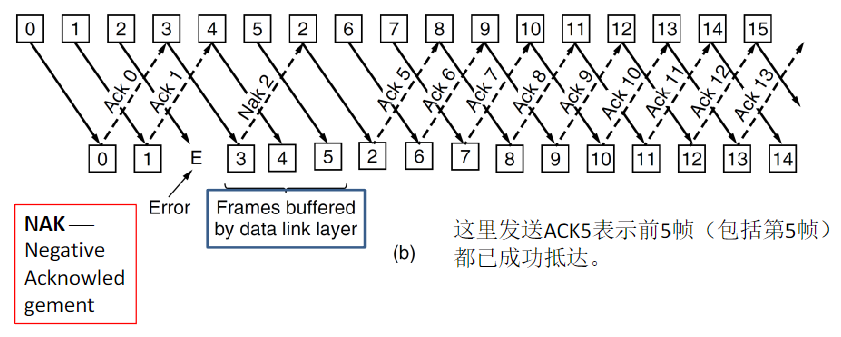
\includegraphics[width=0.42\textwidth]{pic/CN3/Receiver's window size is large.}
    \caption{Receiver's window size is large. --- Selective Repeat}
    \label{fig:Selective Repeat}
\end{figure}

In \textbf{Figure} \ref{fig:Selective Repeat}, a bad frame is received and discarded, but any good frames received after it are accepted and buffered. When the sender times out, only the oldest unacknowledged frame is retransmitted.

\paragraph{Assumptions}:
\begin{itemize}
    \item Data in both directions: piggybacking of ACK. (No separate ACK packets)
    \item Noisy channel
    \item Limited stream of data from network layer. (a ``network\_layer\_ready'' event)
\end{itemize}

\paragraph{Protocol}: Tanenbaum 5th edition: Fig. 3.19 %TODO 自己看 P97-

The sender window of size n. The receive window of size 1. 

%TODO P102-103 Normal Case, Damaged or Lost Case

$MAX\_SEQ$+1 distinct sequence numbers $(0, 1, 2, \dots, MAX\_SEQ)$, no more than $MAX\_SEQ$ unacknowledged frames, the sender $window\le MAX\_SEQ$. %TODO P104-105

\begin{figure}[!htb]
    \centering
    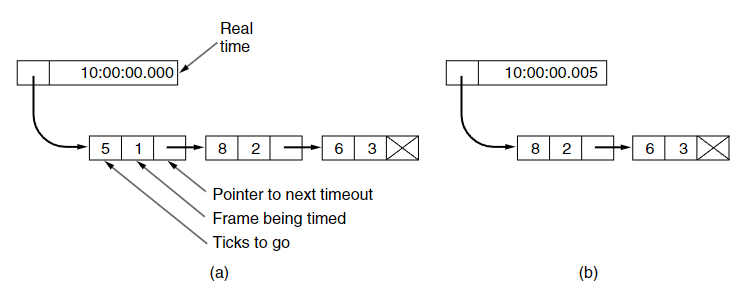
\includegraphics[width=0.42\textwidth]{pic/CN3/Simulation of multiple timers in software}
    \caption{Simulation of multiple timers in software.  (a) The queued timeouts. (b) The situation after the first timeout has expired.}
\end{figure}

\subsubsection{A Sliding Window Protocol Using Selective Repeat}
The selective repeat protocol is to allow the receiver to accept and buffer the frames following a damaged or lost one. 

\paragraph{Assumptions}: 
\begin{itemize}
    \item Data in both directions: piggybacking of ACK. (Separate ACK packets (requires ACK timer), accelerate ack)
    \item Noisy channel
    \item Limited stream of data from network layer
    \item NACK packets: receiver detected problem
\end{itemize}

\paragraph{Protocol}: Tanenbaum 5th Edition Fig. 3.21

%TODO P108-110 摸了
% \begin{enumerate}\small 
%     \item The sender’s window size starts out at 0 and grows to some
%     predefined maximum.
%     \item The receiver’s window, in contrast, is always fixed in size and
%     equal to the predetermined maximum.
%     \item The receiver has a buffer reserved for each sequence number within
%     its fixed window. Associated with each buffer is a bit (arrived) telling
%     whether the buffer is full or empty. Whenever a frame arrives, its
%     sequence number is checked by the function “between” to see if it
%     falls within the window. If so and if it has not already been received, it
%     is accepted and stored.
% \end{enumerate}
Nonsequential receive introduces further constraints on frame sequence number compared to protocols in which frames are only accepted in order!


%TODO e.g. P111-113

%TODO P114-117


\subsection{Examples of data link protocols}
point-to-point lines in the internet in two common situations:
\begin{itemize}
    \item SONET 
    \item ADSL (Asymmetric Digital Subscriber Loop)
\end{itemize}

\subsubsection{Point-to-Point Protocol}
A standard protocol called PPP (Point-to-Point Protocol) is used to send packets over these links.


PPP provides three main features:
\begin{enumerate}
    \item A framing method that unambiguously delineates the end of one frame and the
    start of the next one. The frame format also handles error detection.
    \item A link control protocol for bringing lines up, testing them, negotiating options,
    and bringing them down again gracefully when they are no longer needed. This
    protocol is called LCP (Link Control Protocol).
    \item A way to negotiate network-layer options in a way that is independent of the
    network layer protocol to be used. The method chosen is to have a different
    NCP (Network Control Protocol) for each network layer supported.
\end{enumerate}


\subsubsection{Packet over SONET}
SONET is the physical layer protocol. It provides a bitstream that runs at a well-defined rate. This bitstream is organized as fixed-size byte payloads that recur every 125 $\mu$sec, whether or not there is user data to send.

PPP runs on IP router to provide the transmission mechanism %TODO P123

The PPP frame format %TODO P123


\subsubsection{The PPP Frame Format}
All PPP frames begin with the standard HDLC flag byte of 0x7E (01111110).%TODO P124

\begin{itemize}
    \item The Address field
    \item The Control field
    \item The Protocol field
    \item The Payload field (1500 bytes)
    \item The Checksum field
\end{itemize}

\subsubsection{PPP Link Up \& Down}
%TODO P126

\subsubsection{ADSL (Asymmetric Digital Subscriber Loop)}
%TODO P128


An AAL5 frame %TODO P130

%TDOO 12:13 讲了作业 